\documentclass{ies2018}
\usepackage{amsmath}
\usepackage{graphicx}
\usepackage{algorithm}
\usepackage{algorithmic}
\usepackage{subfigure}
\usepackage[super]{nth}
%% Put title here{}
\title{Novelty Search-based Bat Algorithm: Adjusting Distance among Solutions for Multimodal Optimization}

%% List authors here
\author{Takuya Iwase $^{\dagger}$ \and Ryo Takano $^{\dagger}$ \and Fumito Uwano $^{\dagger}$ \and Hiroyuki Sato $^{\dagger}$ \and Keiki Takadama $^{\dagger}$}
%% Authors' affiliations
\affiliation{%
    ${}^\dagger$ The University of Electro-Communications, Tokyo, Japan\\
    % ${}^\ddagger$ University/Company, City, Country
}
%% Contact email address
\email{tanu_iwa@cas.lab.uec.ac.jp, takano@cas.lab.uec.ac.jp, uwano@cas.lab.uec.ac.jp, h.sato@uec.ac.jp, keiki@hc.uec.ac.jp}

%% Put abstract here
\abstract{%
     % a new algorithm for finding multiple optima in multimodal optimization, which  novelty search-based bat algorithm (NSBA). Conventional algorithms of swarm intelligence tend to straightforward converge a single global optimum or local optimum of high-fitness value. However finding local optima is important because local optima might become better solutions or a new global optimum due to make search domain changed in real world problems. 
    This paper proposes the novelty search-based bat algorithm (NSBA), which aims to search new solutions which have not yet searched to find as many local optima as possible in multimodal optimization.
    In detail, this paper focuses on bat algorithm (BA) which copes with the trade-off between exploration and exploitation in the process of the solution search and extends it by introducing novelty search for keeping the distance among solutions. Through simulations of the comparisons between NSBA and BA in the test-bed multimodal functions, the following implications have been revealed: (1) NSBA finds more number of local optima than BA in both Griewank and Rastrigin Functions; (2) the number of local optima in NSBA increases as the number of populations increases, while that in BA does not change even though the number of populations increases in both functions. 
}%
%% with relevant keywords
\keywords{swarm intelligence, bat algorithm, novelty search, multimodal function}


\begin{document}

\maketitle

\section{Introduction}

Most of metaheuristic algorithms for optimization problems are based on biological evolution as nature-inspired system. For example, Particle Swarm Optimization (PSO) \cite{PSO01} modeled as fish swarm searches solutions by considering both the local best solution of their own fishes and the global best solution among all fishes. Firefly Algorithm (FA) \cite{FA01} searches solutions by moving to a brighter firefly (\textit{i.e.}, better solution). As other algorithm, Bat Algorithm (BA) \cite{BA01} searches solutions according to the characteristic of echolocation which promotes bats to start to find food or prey (\textit{i.e.}, solutions) widely and narrows down the target food or prey by changing their loudness and pulse emission rate. In detail, all bats continuously search solutions by selecting the better solution than the current one, and reduces the number of times of selecting the better solution, which can be found by one of the following three searches: (i) a movement toward the target \textit{i.e.,} the bat which finds the best solution; (ii) a local movement around the target as a local search; and (iii) a random movement as a \textit{global} search. However, all of these algorithms (\textit{i.e.,} PSO, FA and BA) are not appropriate for dealing with real-world problems which need to find many local optima in search space. This is because the above algorithms are designed to find one single global optimum. 

To overcome this problem, this paper focuses on BA and extends it to propose the novelty search-based bat algorithm (NSBA), which aims to search new solutions which have not yet searched to find as many local optima as possible. In this research, BA is employed because of the following reasons: (1) BA based on the three search mechanisms from (i) to (iii) as described above, while PSO and FA is mainly based on one search mechanism (which is respectively based on the local and best solutions in PSO and the movement to better solutions in FA); and (2) this difference suggests that one of search mechanisms in BA can be modified for finding multiple local optima with keeping the two search mechanisms as original, while the search mechanism in PSO and FA are hard to be modified for such a purpose due to a lack of the original search mechanism. What should be noted here is that BA still has the functions of exploitation and exploration in the solution search process as a local search by the mechanism (ii) and a global search by the mechanism (iii). 
% one of metaheuristic algorithms is available to switch exploration and exploitation automatically with characteristic of echolocation . All bats move to single bat which found food or prey, with loudness and pulse rate to sense the distance each other. Simultaneously, some of them fly randomly for searching the other prey globally. After finding a prey, they will drop loudness down and raise pulse rate up automatically, for adjusting to search domain. However considering for dealing with real-world problems which has many multiple optima in search domain, these algorithms are not adaptable because they tend to converge a single global optimum without keeping local optima.
% % Although these algorithms are widely used for optimization problem, the performance of search considerably depends on the scale and contour of multimodal functions. To adapt any optimization problem, we have to consider the balance of performance which unites global search and local search.
 
%  % The bat behavior is determined echolocation which is sound wave for finding food in the dark. Ideally 
%   However, exploitation is still higher performance than exploration, bat algorithm is easily fallen a single global optimum or high-fitness value on multimodal problems. For this reason, we propose distributed BA  for migrating solutions away and keeping distance each other. Besides for the performance measurement, we set different changes: (a) for guiding local search using personal best solution or previous position of solution instead of a global best solution; (b) existence or nonexistence of a new solution generated by flying randomly. 
 % The reasons for multimodal optimization are to find the global optimum definitely, and the other local optima of high-fitness solutions. 
 % There are several approaches for this reasons, which based on Genetic Programming(GP) \cite{GPharada}, PSO \cite{PSO4mo}\cite{PSO4mo2} and Differential Evolutionary(DE) \cite{DE4mo}\cite{DE4mo2}. However, for practical optimization problems, it is desirable to use multimodal functions to reach the peak of both global optima and local optima located, with small population size.  \\

This paper is organized as follows. After this section, the mechanisms of BA and the proposed BA are explained in Sections 2 and 3. Section 4 describes the multimodal functions as the test-bed problem in the experiment. Section 5 shows the results and Section 6 discusses them. Finally, our conclusion is given in Section 7.

\section{Bat Algorithm}
As described in Section 1, BA is a metaheuristic algorithm based on the bat behavior according to its loudness and pulse emission rate of the reflect wave, which control the balance between a local and global search. When a bat finds the better solution than the current one, the loudness $A_i$ and the pulse rate $r_i$ gradually decreases and increases, respectively. To find better solution, the bat has the following three solution search mechanisms: (i) the bat $i$ flies to the target (\textit{i.e.}, the bat which finds the best solution) with the velocity controlled by frequency $f_i$; (ii) the bat $i$ flies around the target as a local search; and (iii) the bat $i$ flies randomly in search space as a global search.
Let us explain these search mechanisms.
First, in the search mechanism (i), all bats change their locations $x_i$ with their velocities $v_i$ toward the global best solution. For this calculation, the frequency $f_i$, velocity $v_i$, and location $x_i$, of the bat $i$ are calculated as follows:
\begin{equation}
f_{i} =f_{min}+(f_{max}-f_{min}) \beta
\label{eq:freq} 
\end{equation}
% \begin{equation}
% d_i^{t-1}=x_*-x_i^{t-1}
% \label{eq:d}
% \end{equation}
\begin{equation}
v_i^t=v_i^{t-1}+(x_*-x_i^{t-1})* f_i
\label{eq:vi}
\end{equation}
\begin{equation}
x_i^t=x_i^{t-1}+v_i^t
\label{eq:xi}
\end{equation}
In detail, the new solution $x_i$ is updated by adding the new the velocity ${v_i}$ which is derived from the previous velocity $v_i^{t-1}$, the distance between the global best location and the previous location $x_*-x_i^{t-1}$, and frequency $f_i$ which range is [${f_{min}}$, ${f_{max}}$] where ${f_{min}}=0$ and ${f_{max}}=1$. $\beta $ is uniform random value from 0 to 1. Next, in the solution search mechanism (ii), the new solution $x_{loc}$ is generated around the global best solution as follows:
\begin{equation}
x_{loc}=x_{*}+ \epsilon A^t \ ,
\label{eq:loc}
\end{equation}
where ${\epsilon}$ is uniform random value between ${[0,  \ 1]}$. In Eq.(\ref{eq:A}), ${A^t}$ is the averaged loudness of all bats. Finally, in the search mechanism (iii), $x_{rnd}$ is generated randomly in search space as follows:
\begin{equation}
\label{eq:xrnd}
x_{rnd}=x_{lb}+(x_{ub}-x_{lb})*rand(1,D)
\end{equation}
where $x_{ub}$ and $x_{lb}$ describe the upper and lower bounds of the search space, and $rand(1,D)$ is the $D$ dimensional uniform random value between $[0, \ 1]$. 

When a bat finds the better solution than the current one, the loudness $A_i$ and pulse emission rate $r_i$ are updated as follows:
\begin{equation}
A_i^{t+1}=\alpha A_i^t
\label{eq:A}
\end{equation}
\begin{equation}
r_i^{t+1}=r_i^0[1-exp(-\gamma t)]
\label{eq:r}
\end{equation}
Note that the loudness $A_i^0$ is initialized as $A_i^0=1$ and the pulse rate is initialized as a uniform random value $r^0$ between $[0, \ 1]$ or a number closed around zero. The parameters $\alpha$ and $\gamma$ are the symbolized damping coefficient. The pseudo code of BA is given in the Algorithm 1 and its brief summary is described below.

\begin{itemize}
\item STEP1: Population initialization of bats (line 1 to 3)\\
The population of bats ${x_i}(i=1, 2, ..., N)$, the loudness ${A_i^0}$, the pulse rate ${r_i^0}$ are initialized as the initial values. The frequency ${f_i}$ is initialized by Eq.(\ref{eq:freq}).
\item STEP2: New solution updates (line 6)\\
The new solutions ${x_i}$ is calculated by Eqs. (\ref{eq:vi})(\ref{eq:xi}).
\item STEP3: New solution generation around global best solution ${x_*}$ (line 7 to 9)\\
A new solution $x_{loc}$ is generated around $x_*$ by Eq. (\ref{eq:loc}) when the pulse emission rate $r_i$ is lower than a random value.
\item STEP4: Random new solution generation (line 10)\\
A new solution ${x_{rnd}}$ is generated randomly by Eq. (\ref{eq:xrnd}).  
\item STEP5: Solutions update(line 11 to 14)\\
When ${rand < A_i}$, the best solution is selected from $x_i$, ${x_{loc}}$, and ${x_{rnd}}$ by Eqs.(\ref{eq:A}),(\ref{eq:r})
\item STEP6: Return to STEP2 
\end{itemize}

\begin{algorithm}[H]
\caption{Bat Algorithm}
\label{code:ba}
\begin{algorithmic}[1]
\REQUIRE Objective\ Function\ $F(x)$
\STATE Initialize Population $x_i(i=1,2,..., N)$ and $v_i$\\
\STATE Define frequency $f_i$ at location $x_i$ [eq.(\ref{eq:freq})]
\STATE Initialize pulse rates $r_i$, and loudness $A_i$
\WHILE{($t <$ Max number of iterations)}
\FOR{i=1 to N}
\STATE Generate a new solution $x_i$ and velocity $v_i$ [eqs.(\ref{eq:vi}) to (\ref{eq:xi})]
\IF{($rand>r_i$)}
\STATE Generate a new solution $x_{loc}$ around a global best solution $x_i$ [eq.(\ref{eq:loc})] 
% \ELSE
% \STATE Continue
\ENDIF
\STATE Generate a new solution $x_{rnd}$ randomly
\IF{($rand<A_i \& \min (F(x_i), F(x_{loc}), F(x_{rnd})<F(x_{i*})$)}
\STATE Accept the new solution, and update pulse rate $r_i$ \\ \& loudness $A_i$ [eqs. (\ref{eq:A})(\ref{eq:r})]  
\ENDIF
\STATE Evaluate all bats and select a best solution $x_*$ in the current solutions
\ENDFOR
\ENDWHILE
\end{algorithmic}
\end{algorithm}

% \section{Distributed Bat Algorithm}
% In this paper, we focus on the distance among population. In Novelty Search-based bat algorithm (NSBA), we consider as written the difference above, and distance of each bat.
% \subsection{k-Nearest Neighbor Bat Algorithm}
% k-nearest neighbor (k-NN) method is used for classification for data with discrete label basically. The mechanism of k-nearest neighbor is to find a new object (a new point) with closest distance between the other objects around it, and predict discrete label from these factors. Here, we use a new object as a new solution with the distance for keeping each bat away. The distance equation is written as below.

% \begin{equation}
% d_i^{t-1}=\frac{1}{K}\sum_{j=1}^K {(x_{i*}-x_j^{t-1})}
% \label{eq:kd*}
% \end{equation}
% \begin{equation}
% d_i^{t-1}=\frac{1}{K}\sum_{j=1}^K {(x_i^{t-1}-x_j^{t-1})}
% \label{eq:kdi}
% \end{equation}

% K describes the number of nearest neighbor. In equation (\ref{eq:nd*}), ${x_{i*}}$ means personal best solution. k-NN is very simple method and is easy to implement, but depending on number of neighbors, we have to choose proper k. Pseudo code is described in Algorithm 2.


\section{Proposed Algorithm}

\subsection{Novelty Search}
Novelty search \cite{noveltysearch} developed in the context of computation aims to search new solutions which have not yet searched. For this purpose, novelty search measures the distance among the candidate solutions to evaluate the dense of them and then generates new solutions into sparse area by considering the distance among candidate solutions. The sparseness of the solutions is calculated as follows:
\begin{equation}
\rho(x)=\frac{1}{k}\sum_{i=0}^k dist(x,\mu_i),
\label{eq:nov}
\end{equation}
where ${\rho(x)}$ is the sparseness at the location ${x}$, $k$ is the number of solutions around $x$ in the k-nearest neighbors, and $dist$ ($x$ and $\mu_i$) is the distance between $x$ and $\mu_i$ which is the $i$-th nearest neighbor of $x$. The $\rho(x)$ value indicates the averaged distance between $x$ and solutions around $x$. Fig. \ref{fig:n_dist} shows an example of the case where $k = 3$ (\textit{i.e.}, the number of solutions around the target solution).  where the yellow star indicates the target solution and the red circles indicates the other solutions. In this figure, the yellow solution moves to the sparse area where is far from other three red solutions. 

\begin{figure}[h]
\begin{center}
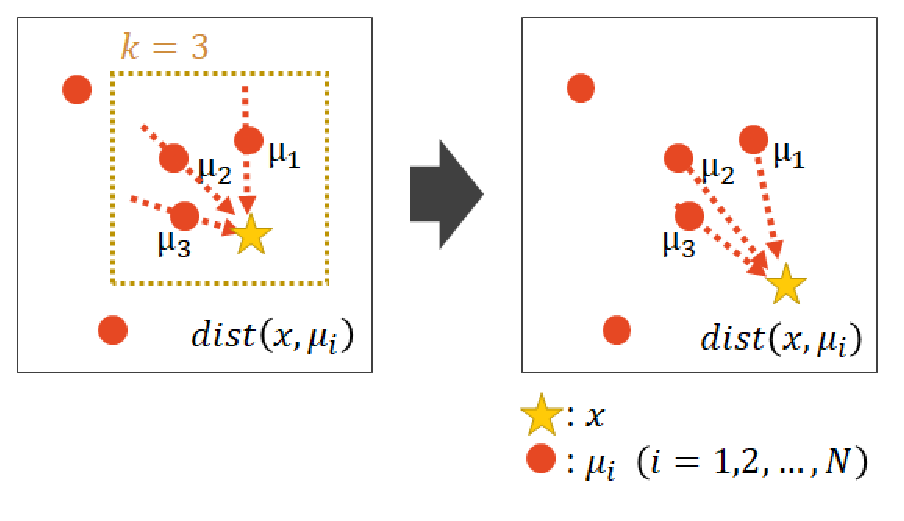
\includegraphics[width=1.0\linewidth]{eps/ns.eps}
\end{center}
\caption{distributed a solution to sparse area}
\label{fig:n_dist}
\end{figure}

\subsection{Novelty Search-based Bat Algorithm}
Novelty Search-based Bat Algorithm (NSBA) is extended from BA by introducing the concept of novelty search, however, we change the value of sparseness equation mentioned above eq.(\ref{eq:nov}) to vector equation. The essential difference between NSBA and BA is related to the search mechanism (i). Concretely, all solutions are updated by adding their velocity calculated by the following Eqs. (\ref{eq:nd*}) and (\ref{eq:nsvi}), which corresponds to Eq. (\ref{eq:vi}) in BA. 
\begin{equation}
d_i^{t-1} = \frac {1}{N} \sum _{j=1}^N \frac {(x_{i*}-x_j^{t-1})}{|x_{i*}-x_j^{t-1}|^2}
\label{eq:nd*}
\end{equation}
\begin{equation}
v_i^t=v_i^{t-1}+d_i^{t-1}*f_i
\label{eq:nsvi}
\end{equation}
where ${N}$ is population size, ${x_{i*}}$ is the current personal best solution, and ${x_i^{t-1}}$ is previous solution. All bats with velocity ${v_i^t}$ and location ${x_i^t}$ are updated same as (\ref{eq:nsvi}) and (\ref{eq:xi}) of BA. Used distance function in Novelty search describes scalar equation. However in this proposes, we alter scalar to vector equation for determining search direction. 
Next, in the search mechanism (ii), $x_{loc}$ is generated around the personal best solution $x_{i*}$ as follows:
\begin{equation}
x_{loc}=x_{i*}+ \epsilon A^t,
\label{eq:ns_xloc}
\end{equation}
where $\epsilon$ is uniform random value between $[0, \ 1]$.
 \subsection{Algorithm of NSBA} 
 The pseudo code of NSBA is given in the Algorithm 2, and its brief summary is described below. Except for the step 2, the other steps are the same as BA.

\begin{itemize}
\item STEP1: Population initialization of bats (line 1 to 3)\\
This step is the same as BA.
\item STEP2: New solution update (line 6)\\
The new solutions ${x_i^t}$ are calculated by Eqs. (\ref{eq:nsvi})(\ref{eq:xi}) with (\ref{eq:nd*}).
\item STEP3: New solution generation around solutions ${x_i}$ (line 7 to 9)\\
 A new solution ${x_{loc}}$ is generated around $x_{i*}$ by Eq. (\ref{eq:ns_xloc})
\item STEP4: Generate a new solution randomly (line 10)\\
This step is the same as BA.
\item STEP5: Solutions update (line 11 to 15)\\
This step is the same as BA.
\item STEP6: Return to STEP2
\end{itemize}

\begin{figure}[h]
\begin{center}
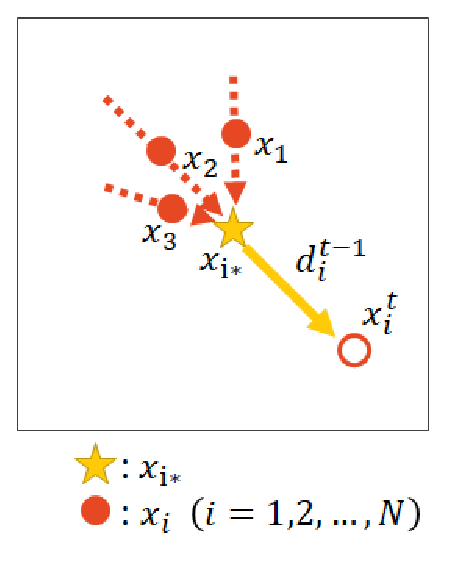
\includegraphics[width=0.5\linewidth]{eps/nsba.eps}
\end{center}
\caption{Bat motion of NSBA}
\label{fig:sbat}
\end{figure}

\begin{algorithm}[H]
\caption{Novelty Search-based Bat Algorithm}
\label{code:sba}
\begin{algorithmic}[1]
\REQUIRE Objective\ Function\ $F(x)$
\STATE Initialize Population $x_i(i=1,2,..., N)$ and $v_i$\\
\STATE Define frequency $f_i$ at location $x_i$ [eq.(\ref{eq:freq})]
\STATE Initialize pulse rates $r_i$, and loudness $A_i$
\WHILE{($t <$ Max number of iterations)}
\FOR{i=1 to N}
\STATE Generate a new solution $x_i$ and update velocity $v_i$  [eqs.(\ref{eq:xi})(\ref{eq:nd*})(\ref{eq:nsvi})] 
\IF{($rand>r_i$)}
\STATE Generate a new solution ${x_{loc}}$ around the solution $x_{i}$ [eq.(\ref{eq:ns_xloc})] 
\ENDIF
\STATE Generate a new solution $x_{rnd}$ randomly (or without ${x_{rnd}}$)
\IF{($rand<A_i \ \& \min (F(x_i), F(x_{new}), F(x_{rnd}))<F(x_{i*})$)}
\STATE Accept the new solution, and update pulse rate $r_i$ \\ \& loudness $A_i$ [eqs. (\ref{eq:A})(\ref{eq:r})] 
\ENDIF
\ENDFOR
\STATE Evaluate the all bats and select a best solution $x_{i*}$ in the current solutions
\ENDWHILE
\end{algorithmic}
\end{algorithm}

\section{Experiment}
To validate the effectiveness of NSBA, this paper employs the following well-known multimodal functions which have similar fitness landscape: Griewank function \cite{f1} and Rastrigin function \cite{f2}.

\subsection{Benchmark Test Functions}
Table. \ref{tab1} summarizes the features of the benchmark multimodal functions. In detail, the first, second, third, and fourth lines indicate the search space, the fitness value of the global optimum, the number of global and local optima, respectively. Figs. \ref{fig:3dgf} \& \ref{fig:3drf} show the fitness landscape of both functions: \ref{fig:cgf} \& \ref{fig:crf} show the contour plot of  both functions from the two-dimensional viewpoint. These figures indicate a change of the fitness value with the color density, where the horizontal and vertical axes indicate $x_1$ and $x_2$, respectively. As a color becomes darker, the fitness value becomes smaller. This paper employs Griewank and Rastrigin functions because both functions are similar fitness landscape but they are some differences of the number of the local optima, search space and fitness value.  

\begin{table}[h]
\caption{Measurement of Benchmark Test Functions}
\begin{center}
\begin{tabular}{c|c|c}
\hline
Function & ${F_1}$ & ${F_2}$ \\
\hline
Search Space & $-10 \leq x_i \leq 10$ & $-5 \leq x_i \leq 5$ \\
% & &  & & \\
\hline
$F(x_*)$ & 0 & 0   \\
\hline
Num of global optima & 1 & 1  \\
\hline
Num of local optima &  16 & 120   \\
\hline
% \multicolumn{4}{l}{$^{\mathrm{a}}$Sample of a Table footnote.}
\end{tabular}
\label{tab1}
\end{center}
\end{table}

 \begin{description}
\item[$F_1$: Griewank Function]\mbox{}\\
This function is described as follows as shown in Fig. \ref{fig:3dgf}.
\begin{equation}
F(x)= \sum_{i=1}^D \frac{x_{i}}{4000} - \prod_{i=1}^D \cos(\frac{x_i}{\sqrt{i}}) + 1,
\end{equation}
where $D$ is the number of dimension and the global optimum is ${f(x_*)}=0$, at $x_* = {[0, \ \ 0]}$. In the case of $D=2$ this function has 17 local optima ${f(x_{i*}) \approx 0}$ at ${\pm x \approx}$ ${ [6.2800, \ \ 8.8769],}$ ${[3.1400, \ \ 4.4385],}$  ${[0, \ \ 8.8769]}$, ${[6.2800 \ \ 0], [9.4200, \ \ 4.4385]}$ in the range between ${-10 \leq x_i \leq 10}$ with $i=1,2$.

\item[$F_2$: Rastrigin Function]\mbox{}\\
 This function is described as follows as shown in Fig. \ref{fig:3drf}.
 \begin{equation}
F(x)= 10D+\sum_{i=1}^D [x_i^2-10 \cos(2\pi x_i)]
\end{equation}
where $D$ is the number of dimension and the global optimum is ${f(x_*)=0}$ at ${x=[0, \ \ 0]}$. In the case of $D=2$, this function has 121 local optima in the search space at ${ \pm x_i=}$ ${[0,...,11 \ \ 0,...,11]}$ in the range between $-5 \leq x_i \leq 5$ with $i=1,2$.

\end{description}

\begin{figure}[h]
\centering
\subfigure[Fitness landscape]{
\includegraphics[width=0.8\linewidth]{eps/3d_griewank.eps}
\label{fig:3dgf}}
\subfigure[Contour plot]{
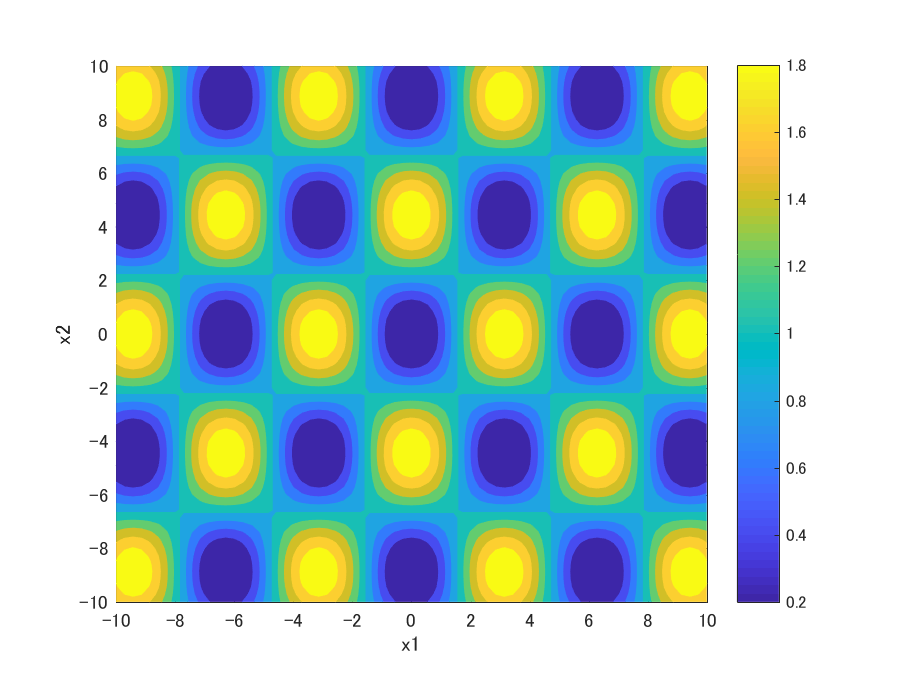
\includegraphics[width=0.8\linewidth]{eps/cont_griewank.eps}
\label{fig:cgf}}

\caption{$F_1$: Griewank Function}
\label{fig:f1}
\end{figure}

\begin{figure}[h]
\centering
\subfigure[Fitness landscape]{
\includegraphics[width=0.8\linewidth]{eps/3d_rastrigin.eps}
\label{fig:3drf}}
\subfigure[Contour plot]{
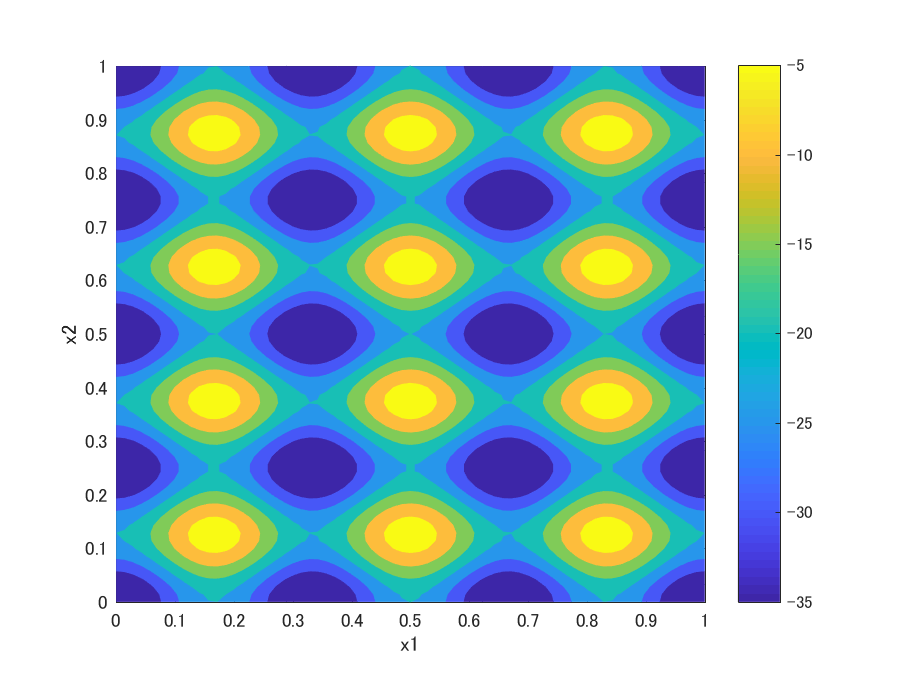
\includegraphics[width=0.8\linewidth]{eps/cont_rastrigin.eps}
\label{fig:crf}}

\caption{$F_2$: Rastrigin Function}
\label{fig:f2}
\end{figure}

\subsection{Evaluation Criteria}
This experiment employs Peak Ratio(PR) \cite{crowdingDE} as the evaluation criterion in the CEC (IEEE Congress on Evolutionary Computation) 2013 competition \cite{cec2013}. The PR value measures the ratio of the found global and local optima in the total number of true peaks and it is calculated as follows: 
\begin{equation}
\label{eq:PR}
PR=\frac{\sum_{run=1}^{MR}FPs}{TP*MR}
\end{equation}
 where ${MR}$ indicates the maximum run, ${FPs}$ indicates  indicates the number of peaks found by the optimization algorithm. ${TP}$ indicates the true number of peaks of the function. We define that the peak is found when the Euclid distance between the true peak and the solution calculated by the optimization algorithm is less than the threshold $\varepsilon = 0.1$.

\subsection{Experimental Parameters}
All experiments employs the parameters as follows: frequency ${f_{max}=1, f_{min}=0}$, loudness ${A^0}=1$, parse rate ${r^0} \in [0, \ 1]$ with ${\alpha =\gamma = 0.9}$. The population size ${N=50,100}$ for Griewank function and $N=100,150$ for Rastrigin function. In both functions, the optimization algorithm runs 30 time, each of which maximum iteration is 10000.

\section{Result and Discussion}
To evaluate NSBA, this paper compares the performance between NSBA and BA in terms of (a) the number and ratio of the found peaks and (b) the convergence speed.

\subsection{Number and Ratio of Found Peaks}
From the viewpoint of the (a) criteria, Table. \ref{tab2} compares both algorithms in terms of the Mean and SD of the number of the found peaks and the PR value of averaged over 30 runs. From this table, NSBA performs better than BA because both the number of the found peaks and the PR value of NSBA is larger than those of BA in both functions with the different population size. Figs. \ref{fig:results_ba} and \ref{fig:results_nsba} show the location of the solutions (marked with the white circle) of both algorithms at the final iteration. BA converged to the single global optimum on any run, while NSBA distributes the solutions to not only the single global optimum but also the other local optima.
% We evaluated each algorithm and compare these performance of convergence speed and the number of found peaks (as shown in Table. \ref{tab2}). From this table, NSBA performed better than BA, reaching some peaks on each function. Fig. \ref{fig:results_ba} \& \ref{fig:results_nsba} show population (marked with white circle) of each algorithm at final iteration. BA converged straightforward to a single global optima on any run. Meanwhile, NSBA distributed population to a single global optima and around it. 
\begin{figure}[t]
\centering
\subfigure[$F_1 :(N=50)$]{
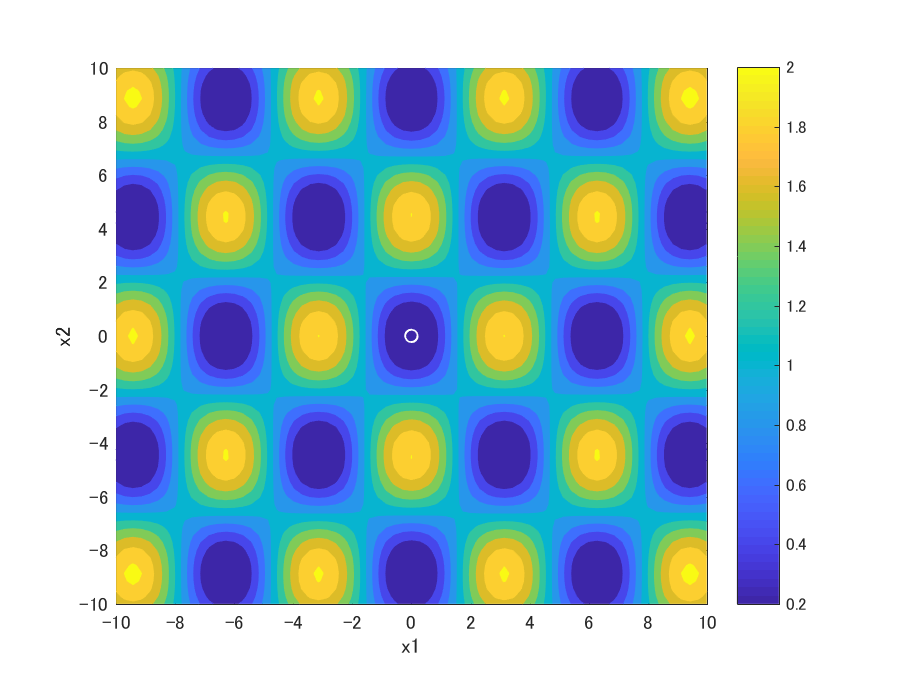
\includegraphics[width=0.8\linewidth]{eps/f1_ba50.eps}
\label{fig:f1_ba50}}
\subfigure[$F_1 :(N=100)$]{
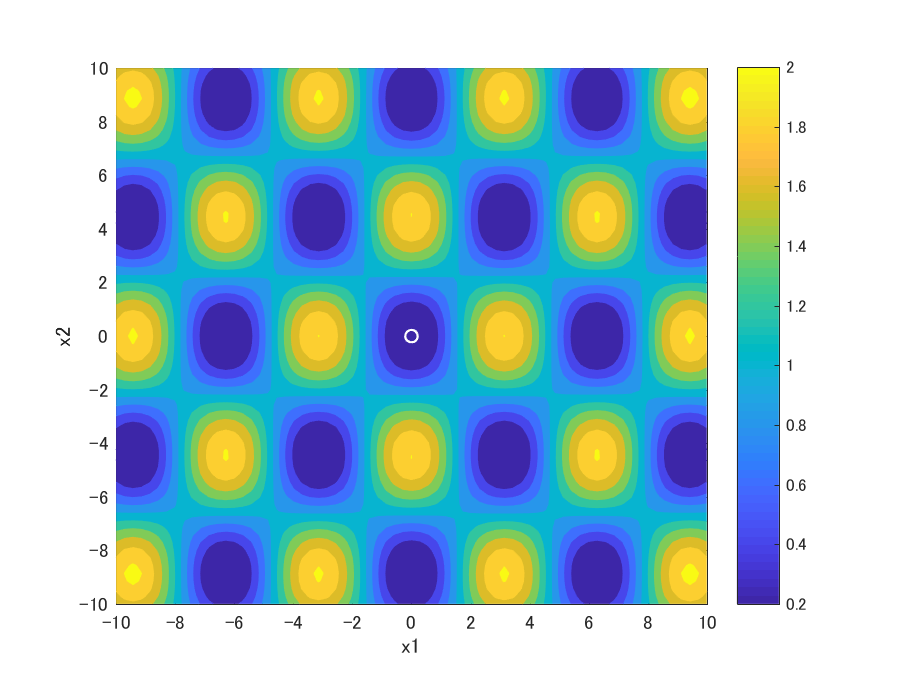
\includegraphics[width=0.8\linewidth]{eps/f1_ba100.eps}
\label{fig:f1_ba100}}
\subfigure[$F_2 :(N=100)$]{
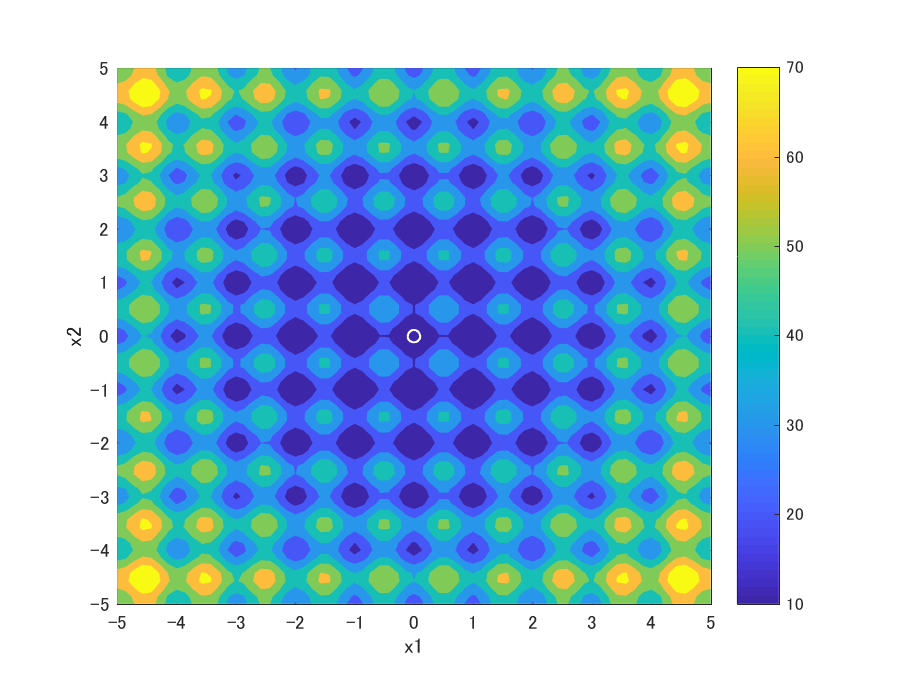
\includegraphics[width=0.8\linewidth]{eps/f2_ba100.eps}
\label{fig:f2_ba100}}
\subfigure[$F_2 :(N=150)$]{
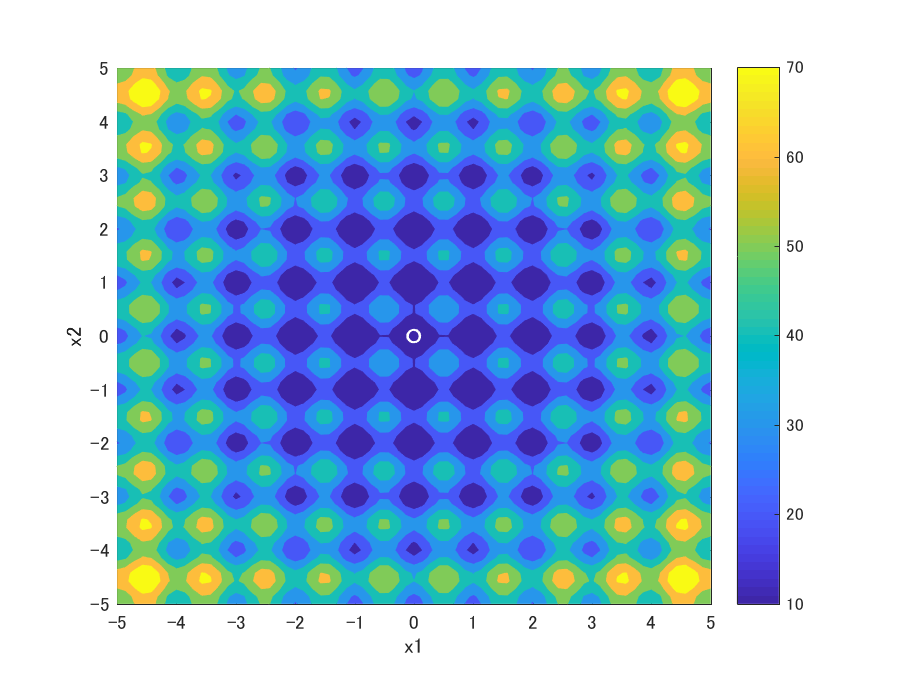
\includegraphics[width=0.8\linewidth]{eps/f2_ba150.eps}
\label{fig:f2_ba150}}

\caption{BA}
\label{fig:results_ba}
\end{figure}

\begin{figure}[b]
\centering
\subfigure[$F_1 :(N=50)$]{
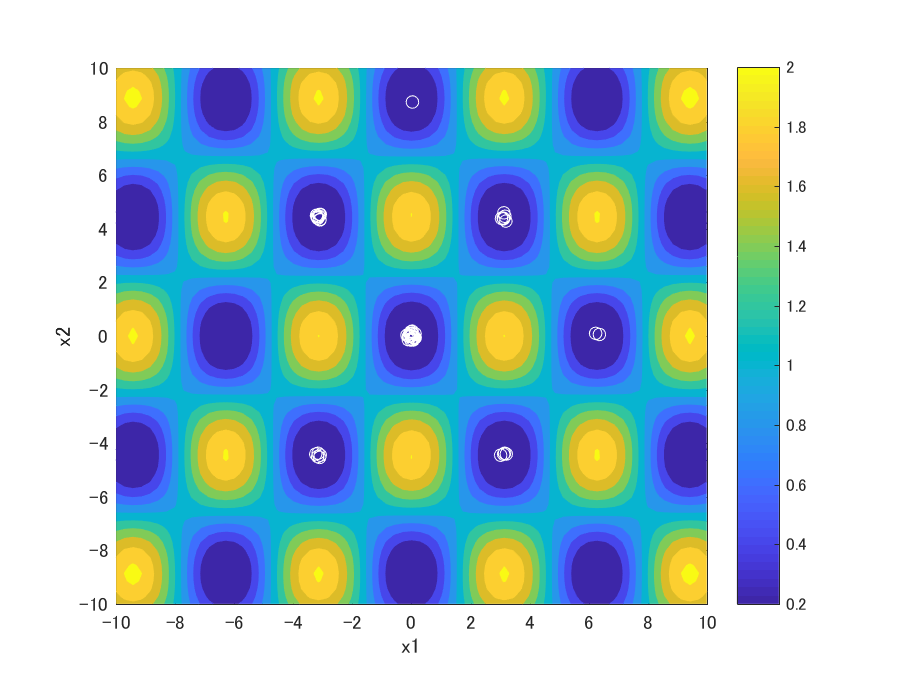
\includegraphics[width=0.8\linewidth]{eps/f1_nsba50.eps}
\label{fig:f1_nsba50}}
\subfigure[$F_1 :(N=100)$]{
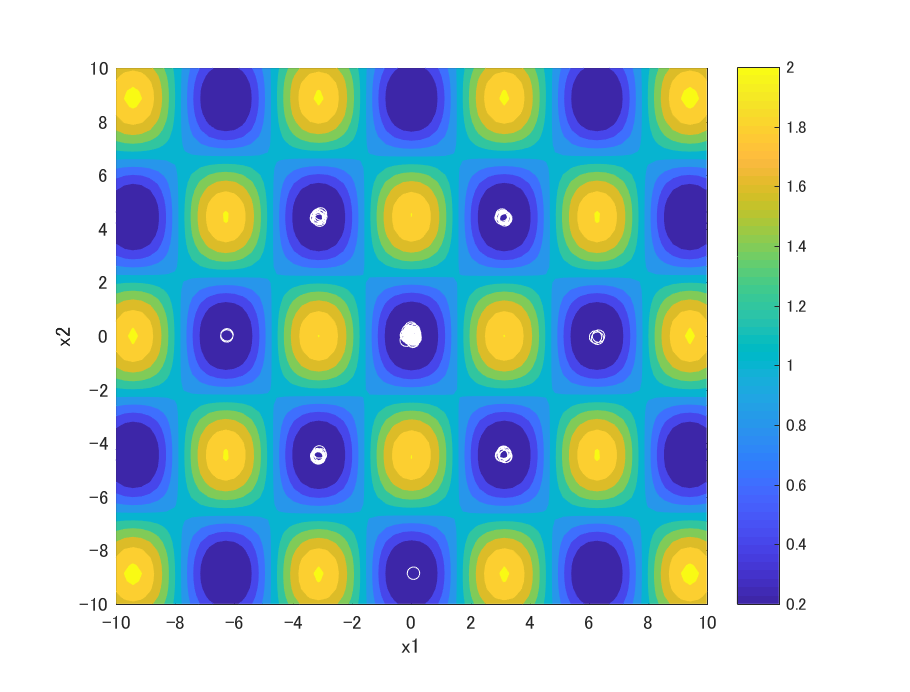
\includegraphics[width=0.8\linewidth]{eps/f1_nsba100.eps}
\label{fig:f1_nsba100}}
\subfigure[$F_2 :(N=100)$]{
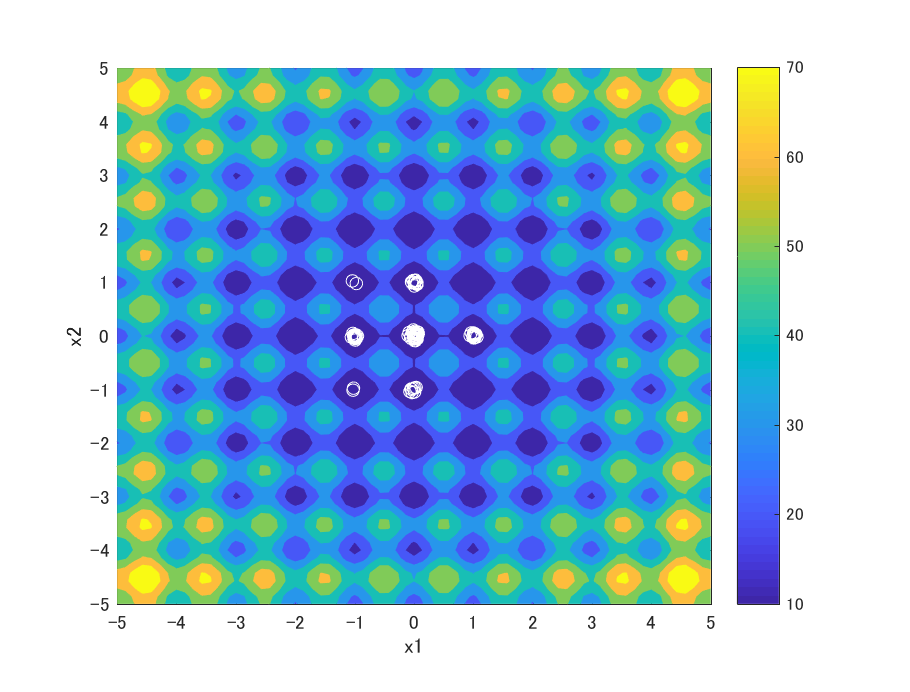
\includegraphics[width=0.8\linewidth]{eps/f2_nsba100.eps}
\label{fig:f2_nsba100}}
\subfigure[$F_2 :(N=150)$]{
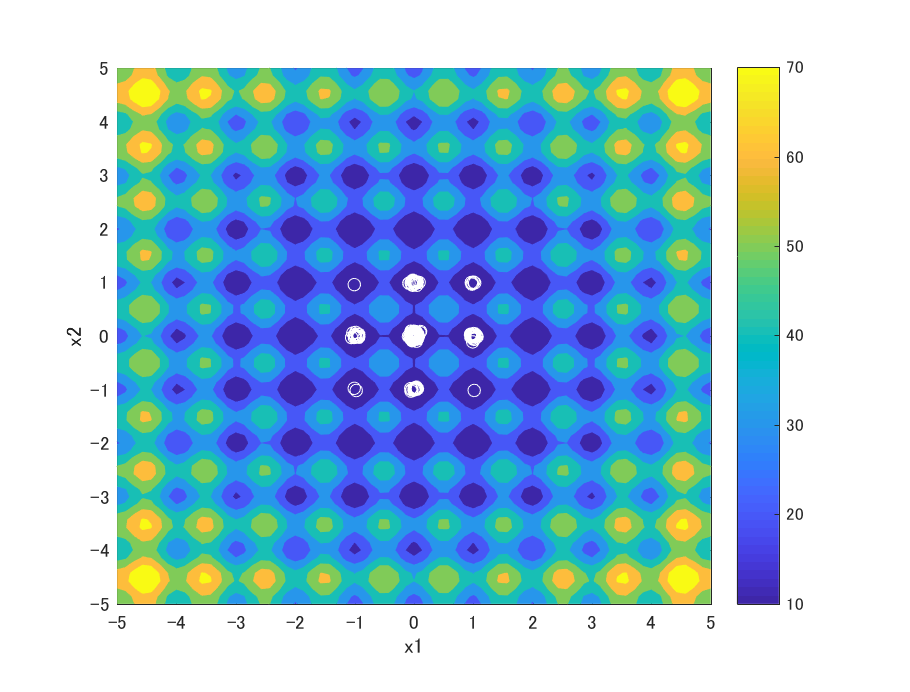
\includegraphics[width=0.8\linewidth]{eps/f2_nsba150.eps}
\label{fig:f2_nsba150}}

\caption{NSBA}
\label{fig:results_nsba}
\end{figure}

\begin{table*}[t]
\caption{Found Peaks and Peak Ratio of BA and NSBA}
\begin{center}
\begin{tabular}{c|c|c|c|c|c|c}
\hline
\multicolumn{1}{c|}{} & \multicolumn{3}{c|}{BA} & \multicolumn{3}{c}{NSBA}  \\
\hline
Function & Mean & SD & PR & Mean & SD & PR \\
\hline
$F_1 \ (N=50)$ & 1.0 & 0 & 5.89 \% & 6.8 & 0.7024 & 40.0 \% \\
\hline
$F_1 \ (N=100)$ & 1.0 & 0 & 5.89 \% & 7.267 & 0.5735 & 42.75 \% \\
\hline
$F_2 \ (N=100)$ & 1.0 & 0 & 0.87 \% & 7.9333 & 0.8929 & 6.56 \% \\
\hline
$F_2 \ (N=150)$ & 1.0 & 0 & 0.87 \% & 8.0667 & 0.7717 & 6.67 \% \\
\hline
\end{tabular}
\label{tab2}
\end{center}
\end{table*}

% \section{Discussion}
% There are line graphs for all methods on Griewank function. The horizontal axis describes iteration of evaluating solutions, and vertical axis describes the sum of distance between each local optima and the closest solution shown as Fig. \ref{fig:ri*_iter} to \ref{fig:it_iter}. Besides distributed solutions at 1000th iteration from Fig. \ref{fig:1000_15} and \ref{fig:1000_26} for rastrigin function from Fig. \ref{fig:1000_37} and \ref{fig:1000_48} for griewank function. 
% \subsection{k-NNBA vs NSBA}
% From Fig. \ref{fig:rtbar_func} to \ref{fig:tbar_func}, k-NNBA tends to decline as neighbors increase. NSBA is hardly affected by changes of neighbors, so that it performed better than k-NNBA relatively. Especially in k=4 from Fig. \ref{fig:1000_15}, \ref{fig:1000_26} and \ref{fig:1000_48}, k-NNBA more distributed than NSBA obviously. It means that equation of considering distance still performed weakly. For this reason, we have to adjust the number of neighbors and population size and updating equation.
  
% \subsection{Existence or nonexistence of ${x_{rnd}}$}
% Compared line graph with Fig. \ref{fig:ri*_iter} \& \ref{fig:rit_iter} and Fig. \ref{fig:i*_iter} \& \ref{fig:it_iter}, ${x_{rnd}}$ affected iteration. Especially in Fig. \ref{fig:ri*_iter} \& \ref{fig:it_iter}, ${dist}$ fluctuated until 1000 iterations in any neighbors. By contrast in Fig. \ref{fig:i*_iter} \& \ref{fig:it_iter}, ${dist}$ of any neighbors became stable over a certain iteration. 

% \subsection{Differences in ${x_i^{t-1}}$ and ${x_{i*}}$}
% Focused on 4 line graphs in right side Fig. \ref{fig:i*_iter} and \ref{fig:it_iter} without ${s_{rnd}}$, ${x_{i*}}$ indicates personal best solution, these ${dist}$ fell continuously until 300 iterations and became stable to the end. From left side in Fig. \ref{fig:ri*_iter} \& \ref{fig:rit_iter}, all ${dist}$ fluctuated constantly, as ${x_{rnd}}$ has strong effect on iteration.

\subsection{Convergence Speed}
From the viewpoint of the (b) criteria, Fig. \ref{fig:all_iter} measures the convergence speed of the peak ratio (PR) of NSBA and BA. In this figure, the vertical axis indicates the peak ratio while horizontal axis indicates the iteration. The lines with the black and while circle indicate the PR value of NSBA and BA, respectively. As shown in Fig. from \ref{fig:f1_ba50} to \ref{fig:f2_ba150}, the PR value in BA sharply decreases to almost 0 \% until 1000 iterations and keeps the same value in both functions. In comparison with the BA, the PR value of NSBA in $F_1$ increases around 70 \% until 1000 iterations and then gradually decreases to around 30-50 \% after 1000 iterations. However, the PR value of NSBA in $F_2$ does increase but gradually decreases from 20 \% to 10 \% after 1000 iterations. This results suggests that the search mechanism (ii) works to spread solutions away toward sparse area, however, NSBA has strong convergence to the global best solution and the personal best solutions around it. 
% \begin{figure*}[t]
% \begin{tabular}{cccc}

% \renewcommand{\thefigure}{\alph{figure}}
% \setcounter{figure}{0}
% \begin{minipage}{0.24\hsize}
% \centering
% 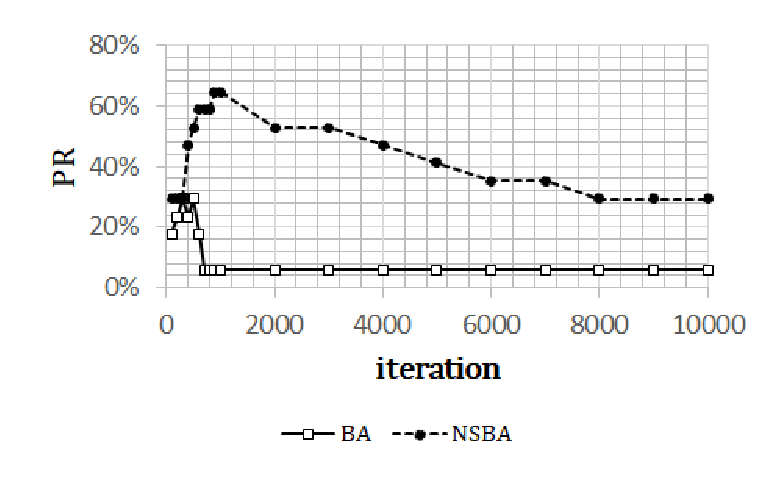
\includegraphics[width=1.0\linewidth]{eps/f1_n50.eps}
% \caption{$F_1 :(N=50)$}
% \label{fig:f1_n50}
% \end{minipage} 

% \begin{minipage}{0.24\hsize}
% \centering
% 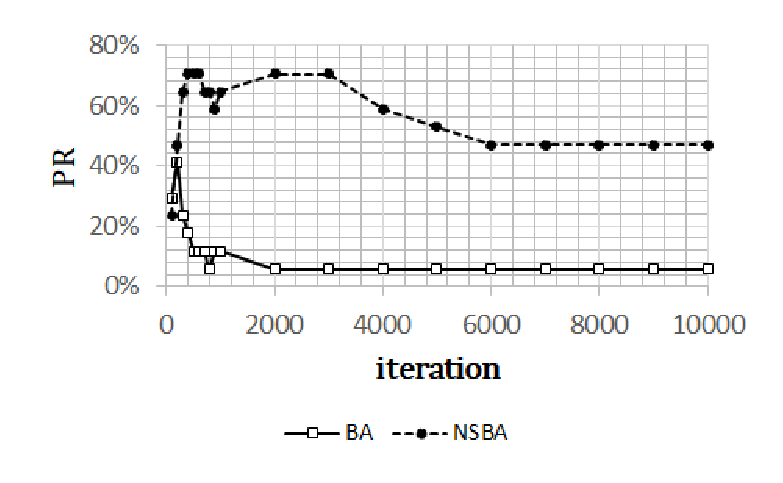
\includegraphics[width=1.0\linewidth]{eps/f1_n100.eps}
% \caption{$F_1 :(N=100)$}
% \label{fig:f1_n100}
% \end{minipage} 

% \begin{minipage}{0.24\hsize}
% \centering
% 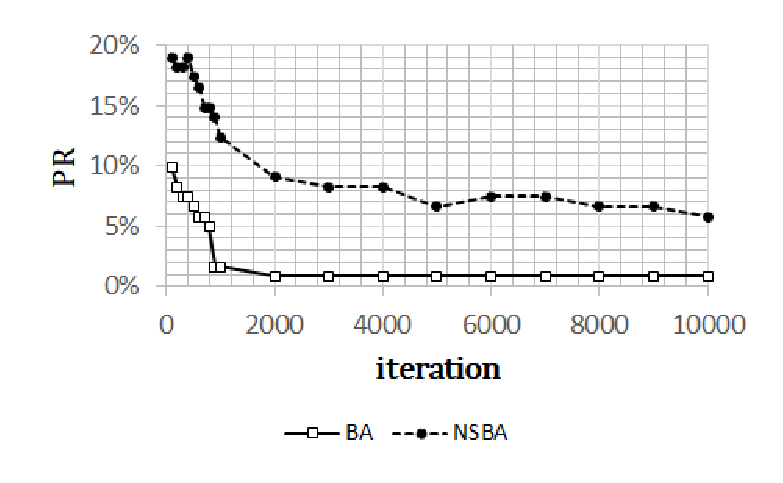
\includegraphics[width=1.0\linewidth]{eps/f2_n100.eps}
% \caption{$F_2 :(N=100)$}
% \label{fig:f2_n100}
% \end{minipage} 

% \begin{minipage}{0.24\hsize}
% \centering
% 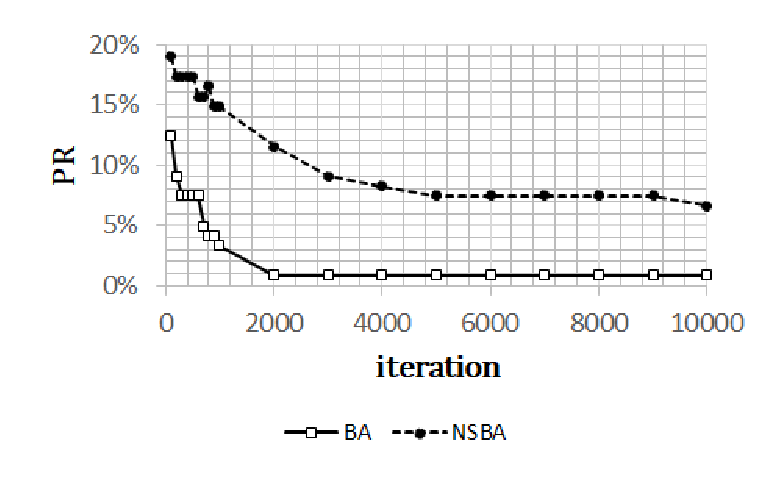
\includegraphics[width=1.0\linewidth]{eps/f2_n150.eps}
% \caption{$F_2 :(N=150)$}
% \label{fig:f2_n150}
% \end{minipage}

% \end{tabular}
% \setcounter{figure}{6}
% \caption{Convergence Speed of Peak Ratio implemented by BA and NSBA}
% \label{fig:all_iter}
% \end{figure*}

\begin{figure}[pt]
\centering
\subfigure[$F_1 :(N=50)$]{
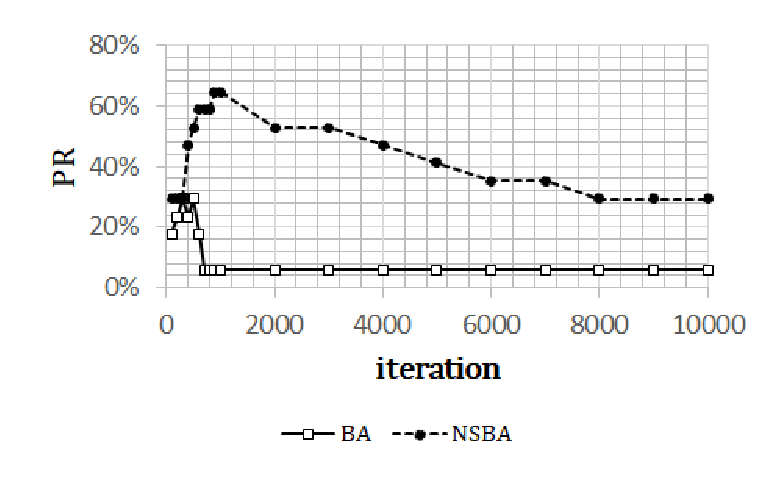
\includegraphics[width=0.8\linewidth]{eps/f1_n50.eps}
\label{fig:f1_n50}}
\subfigure[$F_1 :(N=100)$]{
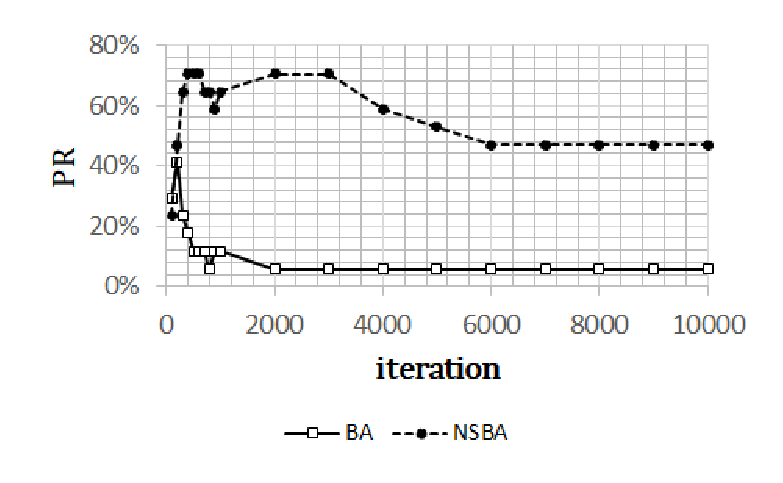
\includegraphics[width=0.8\linewidth]{eps/f1_n100.eps}
\label{fig:f1_n100}}
\subfigure[$F_2 :(N=100)$]{
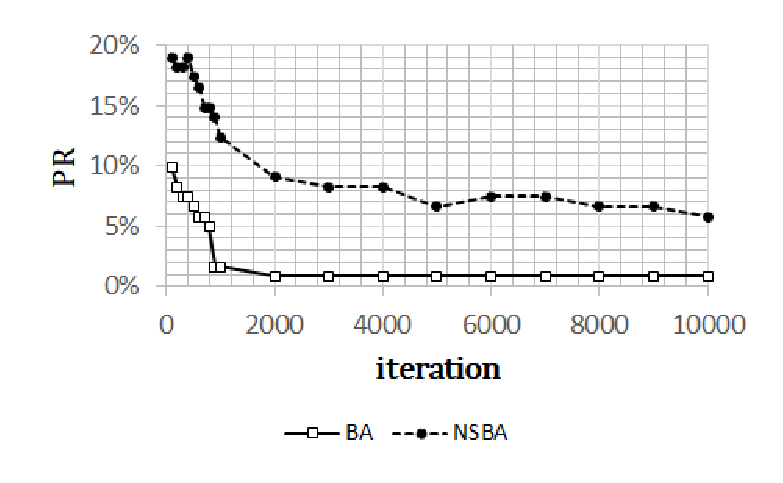
\includegraphics[width=0.8\linewidth]{eps/f2_n100.eps}
\label{fig:f2_n100}}
\subfigure[$F_2 :(N=150)$]{
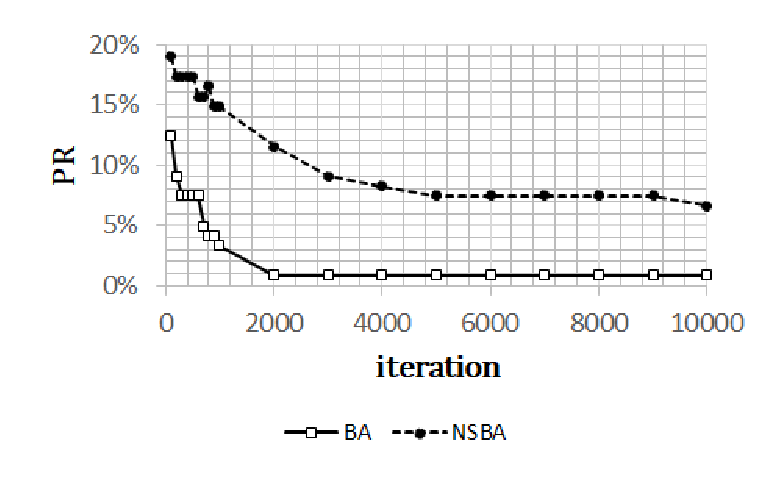
\includegraphics[width=0.8\linewidth]{eps/f2_n150.eps}
\label{fig:f2_n150}}

\caption{Convergence Speed of Peak Ratio implemented by BA and NSBA}
\label{fig:all_iter}
\end{figure}

\subsection{Analysis of Results}
\subsubsection{Population Size}
In order to investigate the influence of the population size, this subsection analyzes the results of BA and NSBA in the different population size. From Table \ref{tab2}, the number of the found peaks and the PR value of BA do not change by the different population size in both functions, while those of NSBA increase as the population size increases. Concretely, the number of the found peaks and the PR value of NSBA increase from 6.8 and 40 \% (with 50 population size) to 7.267 and 42.75 \% (with 100 population size) in $F_1$ and from 7.9333 and 6.56 \% (with 100 population size) to 8.0667 and 6.67 \% (with 150 population size) in $F_2$. This results suggests that the large size of the population contributes to increasing the performance of NSBA while does not contributes to BA because the distributed solutions by NSBA can cover many local optima as the population size increases, while the converged solution by BA mainly cover the only global optimum even though the population size increases. Fig. \ref{fig:all_iter} also supports the above good/bad influence of the population size in NSBA, \textit{i.e.}, the PR value of NSBA in $F_1$ decreases from 70 \% to 30 \% in the case of the small (50) population size, while that in $F_1$ keeps around 50 \% after 6000 iterations in the case of the large (100) population size.
\begin{figure}[pb]
\centering
\subfigure[$F_1 :(N=50)$]{
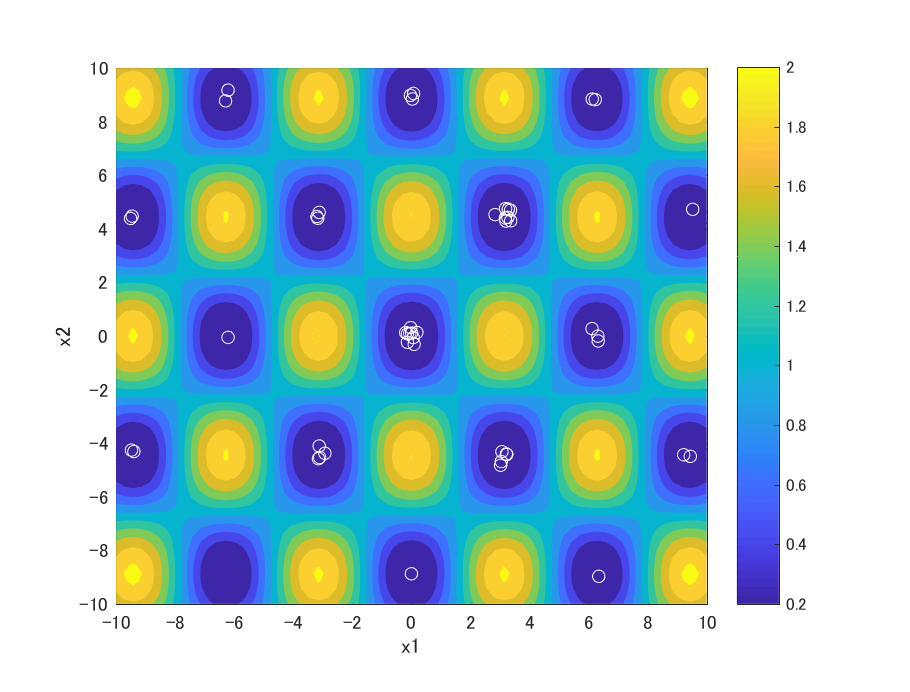
\includegraphics[width=0.8\linewidth]{eps/f1_n50_1000.eps}
\label{fig:f1_n50_1000}}
\subfigure[$F_1 :(N=100)$]{
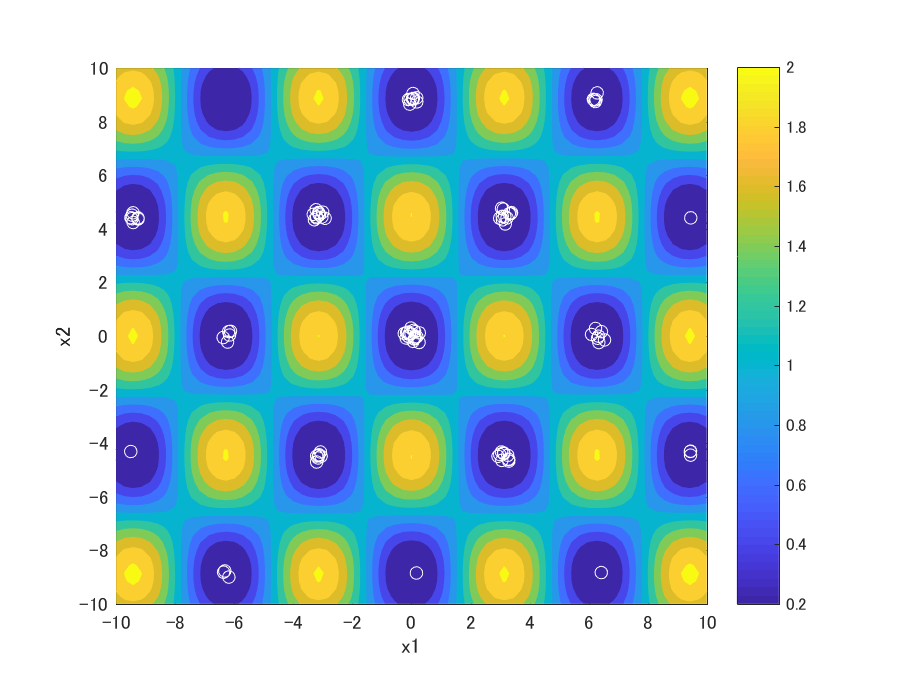
\includegraphics[width=0.8\linewidth]{eps/f1_n100_1000.eps}
\label{fig:f1_n100_1000}}
\subfigure[$F_2 :(N=100)$]{
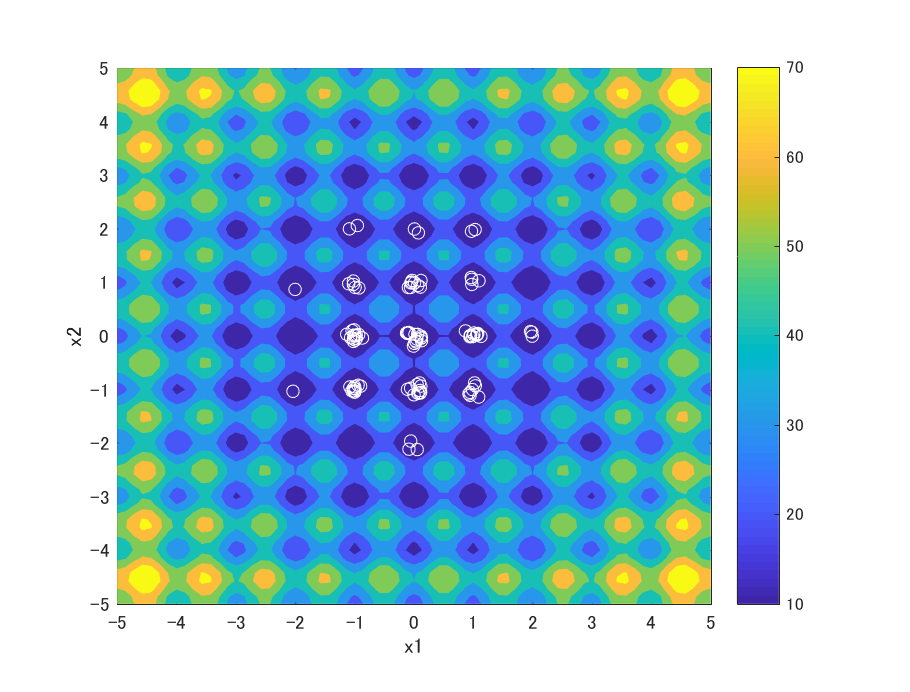
\includegraphics[width=0.8\linewidth]{eps/f2_n100_1000.eps}
\label{fig:f2_n100_1000}}
\subfigure[$F_2 :(N=150)$]{
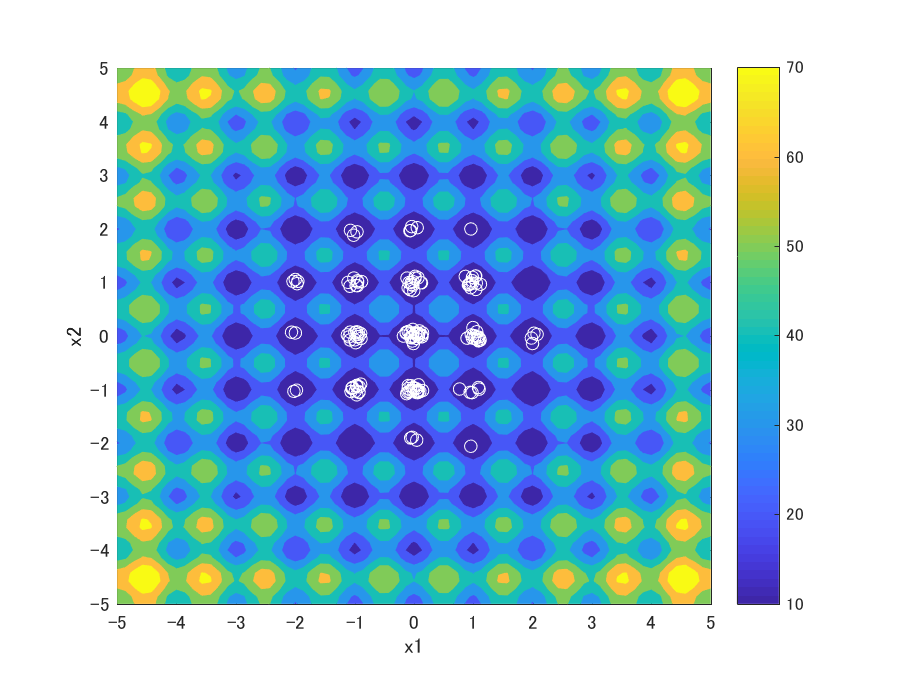
\includegraphics[width=0.8\linewidth]{eps/f2_n150_1000.eps}
\label{fig:f2_n150_1000}}

\caption{Distribution of population of NSBA at 1000 iteration }
\label{fig:results_nsba_1000}
\end{figure}

\subsection{Distribution of Solutions}
In order to investigate the reason why the PR values of NSBA in both function decreases in Fig. \ref{fig:all_iter} (\textit{i.e.} why NSBA cannot keep the maximum PR value), this subsection analyzes how the solutions are distributed in Fig.8 which shows the location of the solutions in 2D dimension at the 1000 iterations. From Fig. \ref{fig:results_nsba_1000}, NSBA can cover almost all peaks at the 1000 iterations on $F_1$ but the number of the found peaks decreases after the 1000 iterations. This because NSBA has the strong convergence to the best solution in the evolutionary process, even though NSBA has a potential of finding the global optimum and many local optima. The same tendency of the decrease of the found peaks can be found in $F_2$ even though the shape of the PR value is different.

\section{Conclusions}
This paper focused on bat algorithm (BA) and extended it to propose the novelty search-based bat algorithm (NSBA), which aims to search new solutions which have not yet searched to find as many local optima as possible in multimodal optimization. Through the comparisons between NSBA and BA in the test-bed multimodal functions, this paper validated the effectiveness of NSBA. Concretely, the following implications have been revealed: (1) although NSBA and BA succeeded to find a global optimum, NSBA found more number of local optima than BA in both Griewank and Rastrigin functions; and (2) the number of local optima in NSBA increased as the number of populations increased, while that in BA did not change even though the number of populations increased in both functions. 
Our future prospects are summarized as follows: (1) applying NSBA into other benchmark functions, and (2) increasing the performance to find the large number of local optima.


% \section{Acknowledgments}
% The author would like to thank R. Takano, F. Uwano, H. Sato and K. Takadama
\begin{thebibliography}{99}
\bibitem{PSO01}
R. Eberhart, J. Kennedy: A New Optimizer Using Particle Swarm Theory,
\textit{Proc. Sixth International Symposium on Micro Machine and Human Science (Nagoya, Japan), IEEE Service center, Pis-cataway, NJ}, No.~1, pp.~39--43, 1995.
\bibitem{FA01}
X. S. Yang: Firefly Algorithms for Multimodal Optimization,
\textit{in:Stochastic Algorithms: Foundations and Applications, SAGA}, Vol.~5792, pp.~169--178, 2009.

\bibitem{BA01}
X. S. Yang: A Metaheuristic Bat-Inspired Algorithm,
 \textit{in: Nature Inspired Cooperative Strategies for Optimization(NICSO 2010), Springer, Berlin}, Vol.~284, pp.~65--74, 2010.

\bibitem{noveltysearch}
J. Lehman and K. O. Stanley.
\newblock Exploiting open-endedness to solve problems through the search for novelty.
\newblock In {\em ALIFE}, pp. 329--336, 2008.

\bibitem{f1}
M. Molga, and C. Smutnicki, Test functions for optimization needs (2005). Retrieved June 2013, from \url{http://www.zsd.ict.pwr.wroc.pl/files/docs/functions.pdf.}

\bibitem{f2}
H. Pohlheim, GEATbx Examples: Examples of Objective Functions (2005). Retrieved June 2013, from \url{http://www.geatbx.com/download/GEATbx_ObjFunExpl_v37.pdf.}

\bibitem{crowdingDE}
R. Thomsen,"Multimodal Optimization using Crowding-based Differential Evolution," {\it In the IEEE Congress on Evolutionary Computation,}2004. CEC2004, vol.2, pp. 1382-1389, 19-23 June, 2004.

\bibitem{cec2013}
X. Li, A. Engelbrecht, and M. G. Epitropakis, "Benchmark Functions for CEC'2013 Special Session and Competition on Niching Methods for Multimodal Function Optimization", {\it Evol. Comput.} Mach. Learn. Group, RMIT University, Melbourne, VIC, Australia, Tech. Rep., 2013.


% \bibitem{PSO4mo}
% J. H. Seo, C. H. Lim, C. G. Heo, J. K. Kim, H. K. Jung and C. C. Lee: Multimodal Function Optimization Based on Particle Swarm Optimization, \textit{IEEE Transactions on Magnetics},  Vol.42, pp.1095-1098, No.4, 2006.

% \bibitem{PSO4mo2}
% B. Y. Qu, P. Suganthan, and S. Das: A Distance-Based Locally Informed Particle Swarm Model for Multimodal Optimization, \textit{IEEE Transactions on Evolutionary Computation}, Vol.17, pp. 387-402, No.3, 2013.

% \bibitem{DE4mo}
% Thomsen, R.: Multimodal  Optimization using crowding-based differential evolution,
% \textit{IEEE Congress on Evolutionary Computation}, Vol.2, pp.1382--1389, 2004.

% \bibitem{DE4mo2}
% Li, X. : Efficient differential evolution using speciation for multimodal function optimization, \textit{GECCO Proceedings of the 7th annual conference on Genetic and evolutionary computation}, pp.873-880, 2005.

% \bibitem{GPharada}
% S. Yoshida, T. Harada, and R. Thawonmas: Multimodal Genetic Programming by Using Tree Structure Similarity Clustering, \textit{IEEE 10th International Workshop on Computational Intelligence and Applications, (Hiroshima, Japan)}, 2017.
\end{thebibliography}

\end{document}
